\chapter{新物理探索におけるトリガー性能の改善}
\thispagestyle{empty}
\label{chap:6}
\chapref{chap:3}では粒子速度が遅い場合に懸念されるトリガー効率の低下とタイミング判定の重要性を説明した。
本章では速度の遅い粒子に対するタイミング較正に伴ったトリガー性能の評価および新物理探索における新しい解析手法の提案を行う。

\section{長寿命スタウ粒子サンプルのトリガー性能評価}
\chapref{chap:3}で述べたように、SUSY~の~GMSB~モデルによれば、スタウ粒子が速度の遅い長寿命荷電粒子として存在することが予測されている。
Run~2~後半に新たに導入された重い荷電粒子探索用トリガーは、次バンチと識別された速度の遅い粒子に対して感度を持つ。したがってバンチ識別のタイミングが~TGC~検出器の遅延パラメータの影響で変化した場合、トリガー可能な粒子の速度に変化がみられる可能性がある。
本節では、長寿命スタウ粒子のシミュレーションサンプルを用い、重い荷電粒子探索用トリガーにおけるタイミング調整に伴ったトリガー性能についての比較を行う。

\subsection{タイミング較正に伴ったトリガー効率の比較}\label{sec:tribeta}
タイミング較正前後のシミュレーションにおける粒子速度に依存したトリガー効率を\figref{fig:tribeta}に示す。較正前後においてバンチ判定の分布の変化に伴い、トリガーできる$\beta$の領域が変化していることが分かる。これは、タイミング較正によりバンチを判定するタイミングに違いがあることが影響していると示唆される。また、$\beta=1.0$の光速の領域においては較正前後においてトリガー効率に変化はないことが分かる。

また\figref{fig:tript}は横運動量、$\eta$に依存したスタウサンプルに対するトリガー効率を示している。タイミング較正前後における各トリガー効率を比較するとトリガーできている領域に違いがみられる。トリガー領域に違いがみられる原因としては$\beta$方向のトリガー領域の変化によるものであると考えられる。
\figref{fig:tripteta}は$\eta,~\beta$、$p_{\rm{T}},~\beta$および$p_{\rm{T}},~\beta$方向に区分したトリガー事象の分布を示している。グラフからそれぞれの変数に対して依存性がみられ、事象数としてはシミュレーション間において同一のふるまいを示しているが、タイミング較正によりトリガー事象の分布に変化がみられることが分かる。\figref{fig:tript}におけるふるまいの変化は、\figref{fig:tripteta}の中図より$p_{\rm{T}}$と$\beta$の依存性による影響であることが分かる。 
\begin{figure}[tbp]
    \begin{minipage}{0.49\hsize}
    \centering   
    \includegraphics[width=\textwidth,page=2]{img/rec/stau_600_ori.pdf}
    \subcaption{}
    \end{minipage}
    \begin{minipage}{0.49\hsize}
    \centering   
    \includegraphics[width=\textwidth,page=2]{img/rec/stau_600.pdf}
    \subcaption{}
    \end{minipage}
    \caption[スタウ粒子サンプルにおけるタイミング較正前後の速度に依存したトリガー効率の比較]{スタウ粒子サンプルにおけるタイミング較正前後の速度に依存したトリガー効率の比較。赤は横運動量閾値~10~GeV~の~L1~シングルミューオントリガー、青は横運動量閾値~10~GeV~の遅い荷電粒子探索用トリガーのトリガー効率を示す。(a)~較正前のシミュレーション。(b)~較正後のシミュレーション。}\label{fig:tribeta}
\end{figure}
\begin{figure}[tbp]
    \begin{minipage}{0.49\hsize}
    \centering   
    \includegraphics[width=\textwidth,page=4]{img/rec/stau_600_ori.pdf}
    \end{minipage}
    \begin{minipage}{0.49\hsize}
    \centering   
    \includegraphics[width=\textwidth,page=4]{img/rec/stau_600.pdf}
    \end{minipage}\\
    \begin{minipage}{0.49\hsize}
    \centering   
    \includegraphics[width=\textwidth,page=9]{img/rec/stau_600_ori.pdf}
    \end{minipage}
    \begin{minipage}{0.49\hsize}
    \centering   
    \includegraphics[width=\textwidth,page=9]{img/rec/stau_600.pdf}
    \end{minipage}
    \caption[スタウ粒子サンプルにおけるタイミング較正前後の各変数に依存したトリガー効率の比較]{スタウ粒子サンプルにおけるタイミング較正前後の各変数に依存したトリガー効率の比較。左図は較正前、右図は較正後のシミュレーション。上図は横運動量、下図は$\eta$の依存を表している。黒~(●)~は~L1~ミューオントリガー、赤~(●)~は横運動量閾値~10~GeV~の~L1~シングルミューオントリガー、青~(●)~は横運動量閾値~10~GeV~の遅い荷電粒子探索用トリガー、青~(▲)~は~MET~トリガーを要求しない遅い荷電粒子探索用トリガーのトリガー効率を示す。}\label{fig:tript}
\end{figure}
\begin{figure}[tbp]
    \begin{minipage}{0.49\hsize}
    \centering   
    \includegraphics[width=\textwidth,page=16]{img/rec/stau_600_ori.pdf}
    \subcaption{}
    \end{minipage}
    \begin{minipage}{0.49\hsize}
    \centering   
    \includegraphics[width=\textwidth,page=16]{img/rec/stau_600.pdf}
    \subcaption{}
    \end{minipage}\\
    \begin{minipage}{0.49\hsize}
    \centering   
    \includegraphics[width=\textwidth,page=15]{img/rec/stau_600_ori.pdf}
    \subcaption{}
    \end{minipage}
    \begin{minipage}{0.49\hsize}
    \centering   
    \includegraphics[width=\textwidth,page=15]{img/rec/stau_600.pdf}
    \subcaption{}
    \end{minipage}\\
    \begin{minipage}{0.49\hsize}
    \centering   
    \includegraphics[width=\textwidth,page=14]{img/rec/stau_600_ori.pdf}
    \subcaption{}
    \end{minipage}
    \begin{minipage}{0.49\hsize}
    \centering   
    \includegraphics[width=\textwidth,page=14]{img/rec/stau_600.pdf}
    \subcaption{}
    \end{minipage}
    \caption[スタウ粒子サンプルにおけるタイミング較正前後の各変数に依存した事象の比較]{スタウ粒子サンプルにおけるタイミング較正前後の各変数に依存した事象の比較。左図は較正前、右図は較正後のシミュレーション。上図は$\eta$および速度、中図は横運動量および速度、下図は横運動量および$\eta$の依存を表している。黒の四角は事象数、赤は横運動量閾値~10~GeV~の~L1~シングルミューオントリガー、青は横運動量閾値~10~GeV~の遅い荷電粒子探索用トリガーを通過した事象を示す。}\label{fig:tripteta}
\end{figure}

\subsection{粒子質量の違いによるトリガー効率の比較}\label{sec:trimass}
本研究においては、スタウ粒子のシミュレーションサンプルとして、質量が~600~GeV~および~1000~GeV~のサンプルを使用した。タイミング較正後のシミュレーションを利用し、質量の違いによるトリガー効率への影響について考察する。
\figref{fig:tribeta6}は、速度に依存したトリガー効率の変化を比較したものである。スタウ粒子サンプルの質量が異なることで、トリガーできる$\beta$の領域に変化は見られない。各変数における分布のの詳細については\secref{sec:tribeta}での比較の仕方と同様に行う。
\begin{figure}[tbp]
    \begin{minipage}{0.49\hsize}
    \centering   
    \includegraphics[width=\textwidth,page=2]{img/rec/stau_600.pdf}
    \subcaption{}
    \end{minipage}
    \begin{minipage}{0.49\hsize}
    \centering   
    \includegraphics[width=\textwidth,page=2]{img/rec/stau_1000.pdf}
    \subcaption{}
    \end{minipage}
    \caption[質量の異なるスタウ粒子サンプルにおける速度に依存したトリガー効率の比較]{質量の異なるスタウ粒子サンプルにおける速度に依存したトリガー効率の比較。タイミング較正後のシミュレーションを利用している。赤は横運動量閾値~10~GeV~の~L1~シングルミューオントリガー、青は横運動量閾値~10~GeV~の遅い荷電粒子探索用トリガーのトリガー効率を示す。(a)~質量~600~GeV。(b)~質量~1000~GeV。}\label{fig:tribeta6}
\end{figure}
\figref{fig:tript6}の上図から~L1~トリガー全体として取得できる$p_{\rm{T}}$の領域が異なっていることが分かる。これは同じ粒子速度である場合でも、質量が大きくなると$p_{\rm{T}}$の値が大きくなることに由来する。同じ$p_{\rm{T}}$の場合、質量が大きい方が粒子速度が遅くなるため、バンチ判定においては次バンチの割合が大きくなる。
\figref{fig:trietabeta6}に$\eta,~\beta$、$p_{\rm{T}},~\beta$および$p_{\rm{T}},~\eta$に依存したトリガー可能領域と事象数の分布を示す。
\secref{sec:tribeta}のときとは異なり、事象が観測される領域についても変化していることが分かる。
以上の理由により質量が大きいサンプルの方がトリガーできる$p_{\rm{T}}$の領域が$p_{\rm{T}}$の高い方向にシフトしている。
\figref{fig:tript6}の下図では質量差による影響が確認でき$\eta$方向においてもトリガー可能な領域に違いがみられる。

\begin{figure}[tbp]
    \begin{minipage}{0.49\hsize}
    \centering   
    \includegraphics[width=\textwidth,page=4]{img/rec/stau_600.pdf}
    \end{minipage}
    \begin{minipage}{0.49\hsize}
    \centering   
    \includegraphics[width=\textwidth,page=4]{img/rec/stau_1000.pdf}
    \end{minipage}\\
    \begin{minipage}{0.49\hsize}
    \centering   
    \includegraphics[width=\textwidth,page=9]{img/rec/stau_600.pdf}
    \end{minipage}
    \begin{minipage}{0.49\hsize}
    \centering   
    \includegraphics[width=\textwidth,page=9]{img/rec/stau_1000.pdf}
    \end{minipage}
    \caption[質量の異なるスタウ粒子サンプルにおける各変数に依存したトリガー効率の比較]{質量の異なるスタウ粒子サンプルにおける各変数に依存したトリガー効率の比較。左図は質量~600~GeV、右図は質量~1000~GeV~のサンプル。上図は横運動量、下図は$\eta$の依存を表している。タイミング較正後のシミュレーションを利用している。黒~(●)~は~L1~ミューオントリガー、赤~(●)~は横運動量閾値~10~GeV~の~L1~シングルミューオントリガー、青~(●)~は横運動量閾値~10~GeV~の遅い荷電粒子探索用トリガー、青~(▲)~は~MET~トリガーを要求しない遅い荷電粒子探索用トリガーのトリガー効率を示す。}\label{fig:tript6}
\end{figure}
\begin{figure}[tbp]
    \begin{minipage}{0.49\hsize}
    \centering   
    \includegraphics[width=\textwidth,page=16]{img/rec/stau_600.pdf}
    \end{minipage}
    \begin{minipage}{0.49\hsize}
    \centering   
    \includegraphics[width=\textwidth,page=16]{img/rec/stau_1000.pdf}
    \end{minipage}\\
    \begin{minipage}{0.49\hsize}
    \centering   
    \includegraphics[width=\textwidth,page=15]{img/rec/stau_600.pdf}
    \end{minipage}
    \begin{minipage}{0.49\hsize}
    \centering   
    \includegraphics[width=\textwidth,page=15]{img/rec/stau_1000.pdf}
    \end{minipage}\\
    \begin{minipage}{0.49\hsize}
    \centering   
    \includegraphics[width=\textwidth,page=14]{img/rec/stau_600.pdf}
    \end{minipage}
    \begin{minipage}{0.49\hsize}
    \centering   
    \includegraphics[width=\textwidth,page=14]{img/rec/stau_1000.pdf}
    \end{minipage}
    \caption[質量の異なるスタウ粒子サンプルにおける各変数に依存した事象の比較]{質量の異なるスタウ粒子サンプルにおける各変数に依存した事象の比較。左図は質量~600~GeV、右図は質量~1000~GeV~のサンプル。上図は$\eta$および速度、中図は横運動量および速度、下図は横運動量および$\eta$の依存を表している。タイミング較正後のシミュレーションを利用している。黒の四角は事象数、赤は横運動量閾値~10~GeV~の~L1~シングルミューオントリガー、青は横運動量閾値~10~GeV~の遅い荷電粒子探索用トリガーを通過した事象を示す。}\label{fig:trietabeta6}
\end{figure}

\section{速度に依存したトリガー効率の新しい見積もり手法の構築}\label{sec:est}
\secref{sec:tribeta}、\secref{sec:trimass}では、シミュレーションを用いて、タイミング較正に伴うトリガー効率への影響およびサンプルの質量の違いに伴うトリガー効率への影響について考察してきた。タイミング較正前後の比較においてはトリガー可能な$\beta$の領域に違いがみられることを示し~TGC~のタイミング判定がトリガー効率の速度依存性に直結することが分かった。

物理解析を行う場合、獲得可能な事象数を見積もるために実験データにおけるトリガー効率を算出することが必要であるが、実験において超対称性粒子は未観測であり直接的なトリガー効率の算出はできない。
本研究では実験データにおけるトリガー効率を見積もるための新たな解析手法を開発した結果を示す。

\subsection{確率分布関数の定義方法}\label{sec:pro}
TGC~検出器では、粒子の信号ごとにバンチ識別を行っている。
光速のミューオンを仮定した場合、ほとんどが基準バンチで判定されるが\chapref{chap:4}でも述べた通り、信号が検出されるタイミングには一定の揺らぎがある。統計的に十分なミューオン事象を~TGC~で検出したとする。以上の場合それぞれのミューオンごとにタイミングの揺らぎがあり検出されるタイミングは異なるが、ヒットのタイミングを時間の関数としてみれば、ある確率分布に従って観測されるということが仮定できる。
この確率分布は、バンチ判定をもとに近似的に決定することができる。\figref{fig:rectune}はタイミング較正を行ったシミュレーションにおけるバンチ判定の分布をもとに定義した確率分布関数である。ゲートとヒットタイミングの関係から算出することが可能である。\subsecref{subsec:cali}では、シミュレーションにおける~M1~ステーションのバンチ判定分布割合について示した。確率分布関数は、この割合に従って定義される。バンチを判定するゲートを設定どおり定義し、得られているバンチ判定分布を満たすように確率分布関数の形を決定する。本研究では確率分布関数を近似的に三角形として定義している。以下で三角形の詳細な定義方法についてまとめる。
\begin{itemize}
\item 前かつ基準バンチ、基準バンチ、基準かつ次バンチの割合を示す $\it{R}_{\rm{p{\land}c}}$, $\it{R}_{\rm{c}}$, $\it{R}_{\rm{c{\land}n}}$ がバンチ判定の分布割合を満たすような三角形を考える。確率分布は~M1~におけるバンチ判定の分布を基準として算出する。
\item 三角形の頂点を決定する~(\figref{fig:rectune}の三角形における上部の頂点)~。頂点は任意の座標で決めることができるが、今回は基準バンチの中心を頂点とした。
\item 決定した頂点を固定した上で、バンチ判定の分布割合を満たすように残りの 2 頂点を決定する。
\end{itemize}
以上の同意のもと三角形を決定すれば、一意に確率分布を定義することができる。ワイヤー、ストリップそれぞれにおいて上記の方法で確率分布を求めることで以降のトリガー効率の算出につなげることができる。

\begin{figure}[tbp]
    \begin{minipage}{0.49\hsize}
    \centering   
    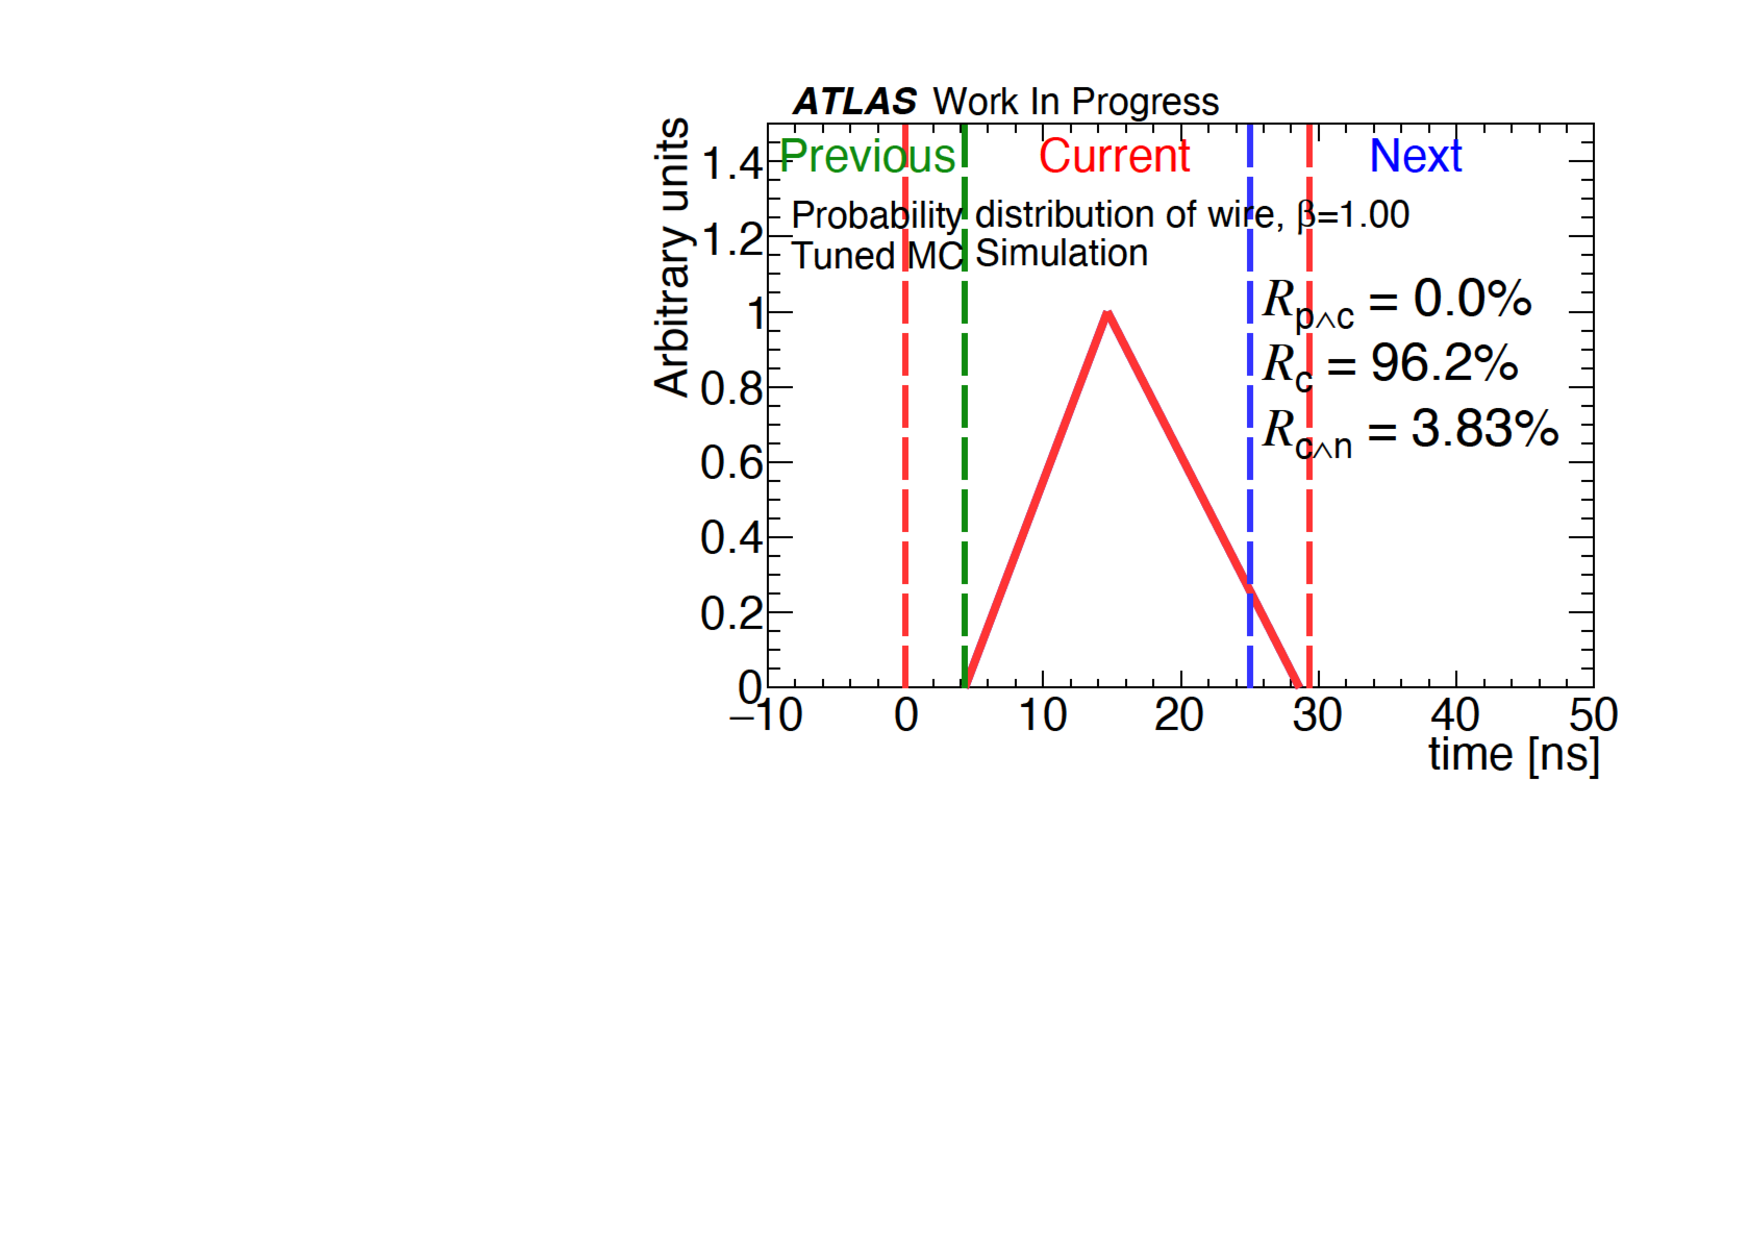
\includegraphics[width=\textwidth,page=1]{img/rec/rec_tune_w.pdf}
    \subcaption{}
    \end{minipage}
    \begin{minipage}{0.49\hsize}
    \centering   
    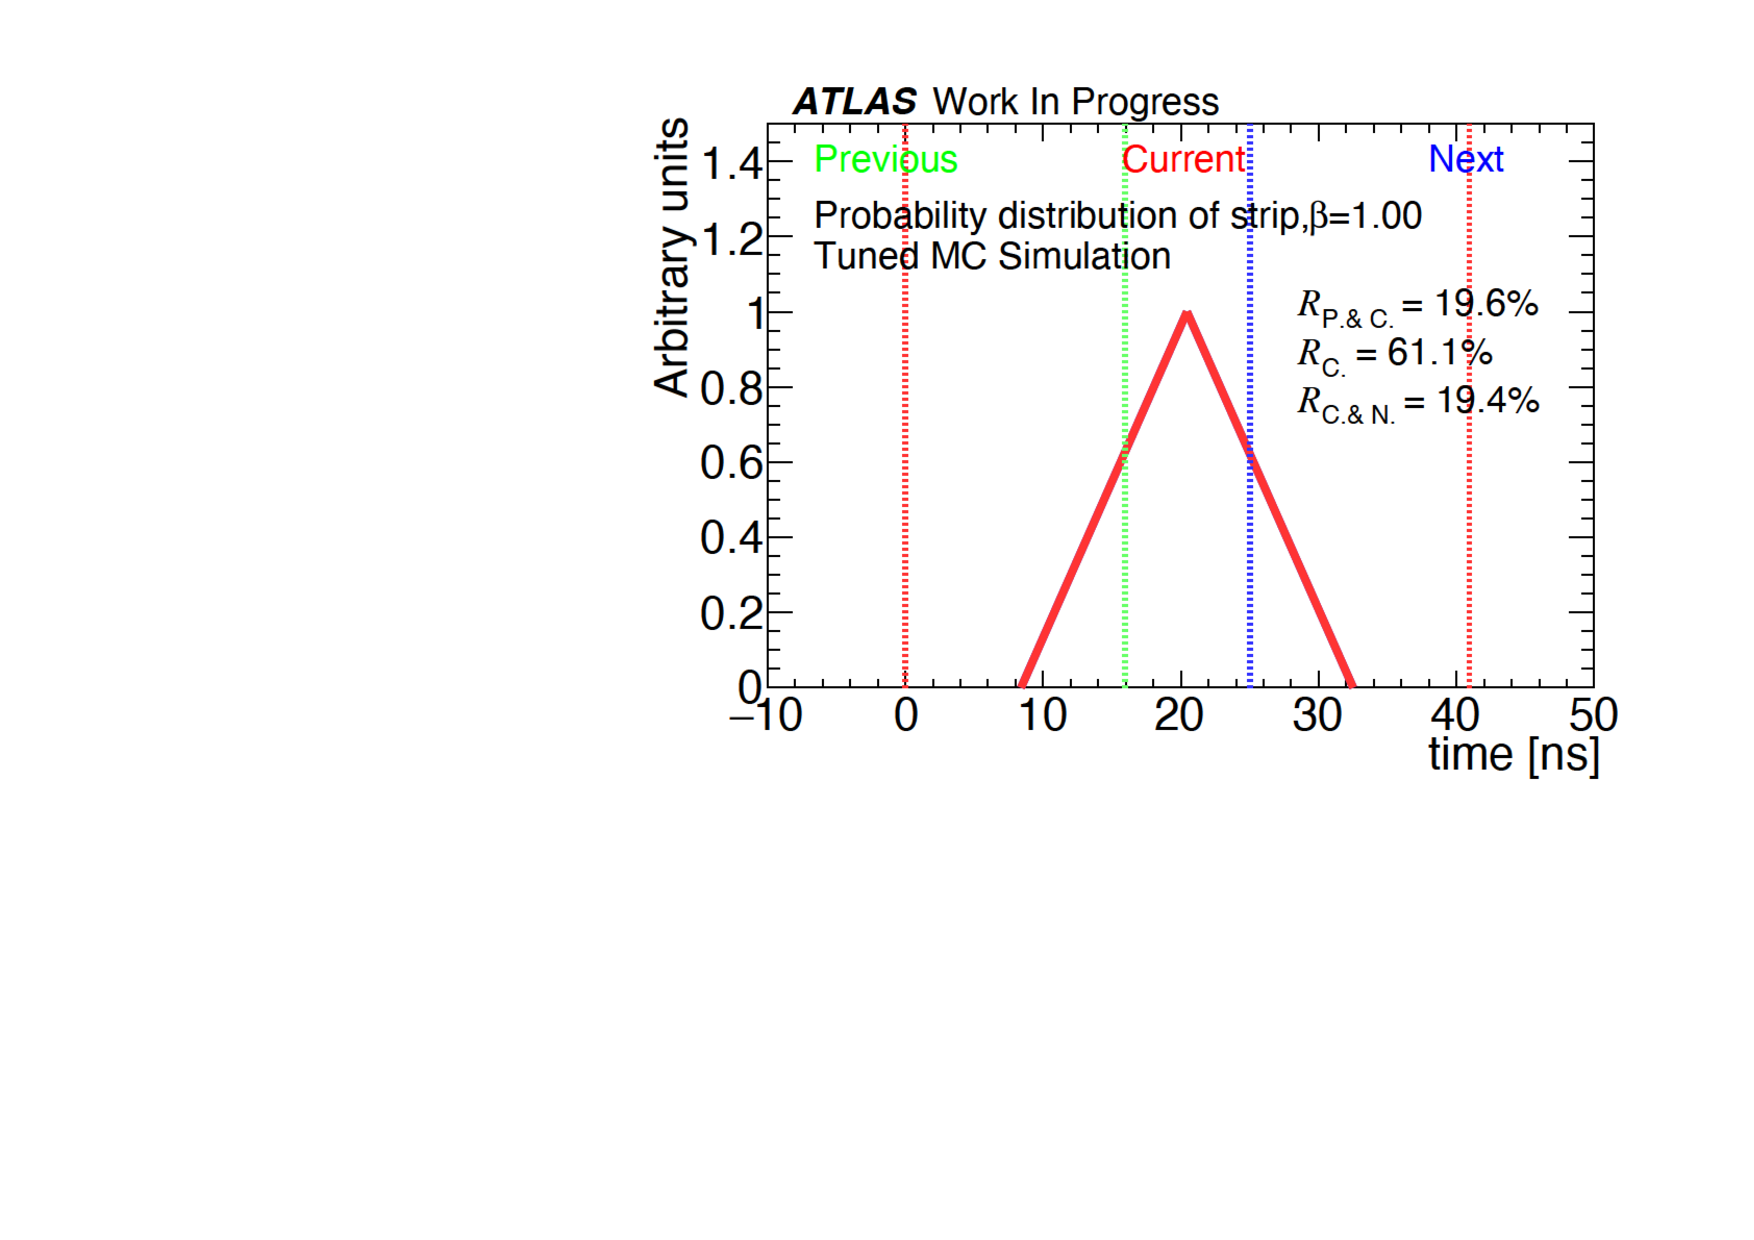
\includegraphics[width=\textwidth,page=1]{img/rec/rec_tune_s.pdf}
    \subcaption{}
    \end{minipage}
    \caption[バンチ判定から推定した較正後のシミュレーションにおけるヒットタイミングの確率分布]{バンチ判定から推定した較正後のシミュレーションにおけるヒットタイミングの確率分布。$R_{\rm{p{\land}c}},~R_{\rm{c}},~R_{\rm{c{\land}n}}$はそれぞれ前かつ基準バンチ、基準バンチ、基準かつ次バンチの確率分布における割合を示している。(a)~M1ワイヤーチャンネル。(b)~M1ストリップチャンネル。}\label{fig:rectune}
\end{figure}

\subsection{粒子速度と確率分布}\label{sec:prob}
前節で求めた確率分布関数は$\beta=1.0$のミューオンの確率分布であると考えることができる。速度の遅い粒子における確率分布を考える場合は、上記のミューオンに対してどれだけ遅れているかという指標をもとに算出することができる。例えば、TGC~の任意のチェンバーに対して速度の遅い粒子が到達する場合を仮定する。このとき、速度の遅い粒子と光速の粒子の同じ場所での到達時間差が計算上、$t$であったとする。すると任意のチェンバーに対する速度の遅い粒子の確率分布は、光速のミューオンの確率分布を$t$だけ遅らせたものであると考えられる。以上の仮定をもとに粒子速度と到達時間の関係から速度の遅い粒子の確率分布を見積もる。

粒子の飛来時間は~TGC~の位置と飛来する角度によって異なる。そこで\figref{fig:velo}に示すように飛来時間が短い~M1~と飛来時間が長い~M3~での角度ごとによる粒子の到達時間を考え、確率分布を見積もった。角度に関しては、エンドキャップ領域において$\eta$を~0.1~毎に分割して考え、各角度での粒子到達時間を計算した。\figref{fig:recbeta}は任意の角度方向において粒子速度の変化により確率分布がどのように変化するかを表した図である。M1~と~M3~での確率分布を算出し両者の確率のかけ合わせにより、トリガーできる割合を見積もる。
\begin{figure}[tbp]
    \centering   
    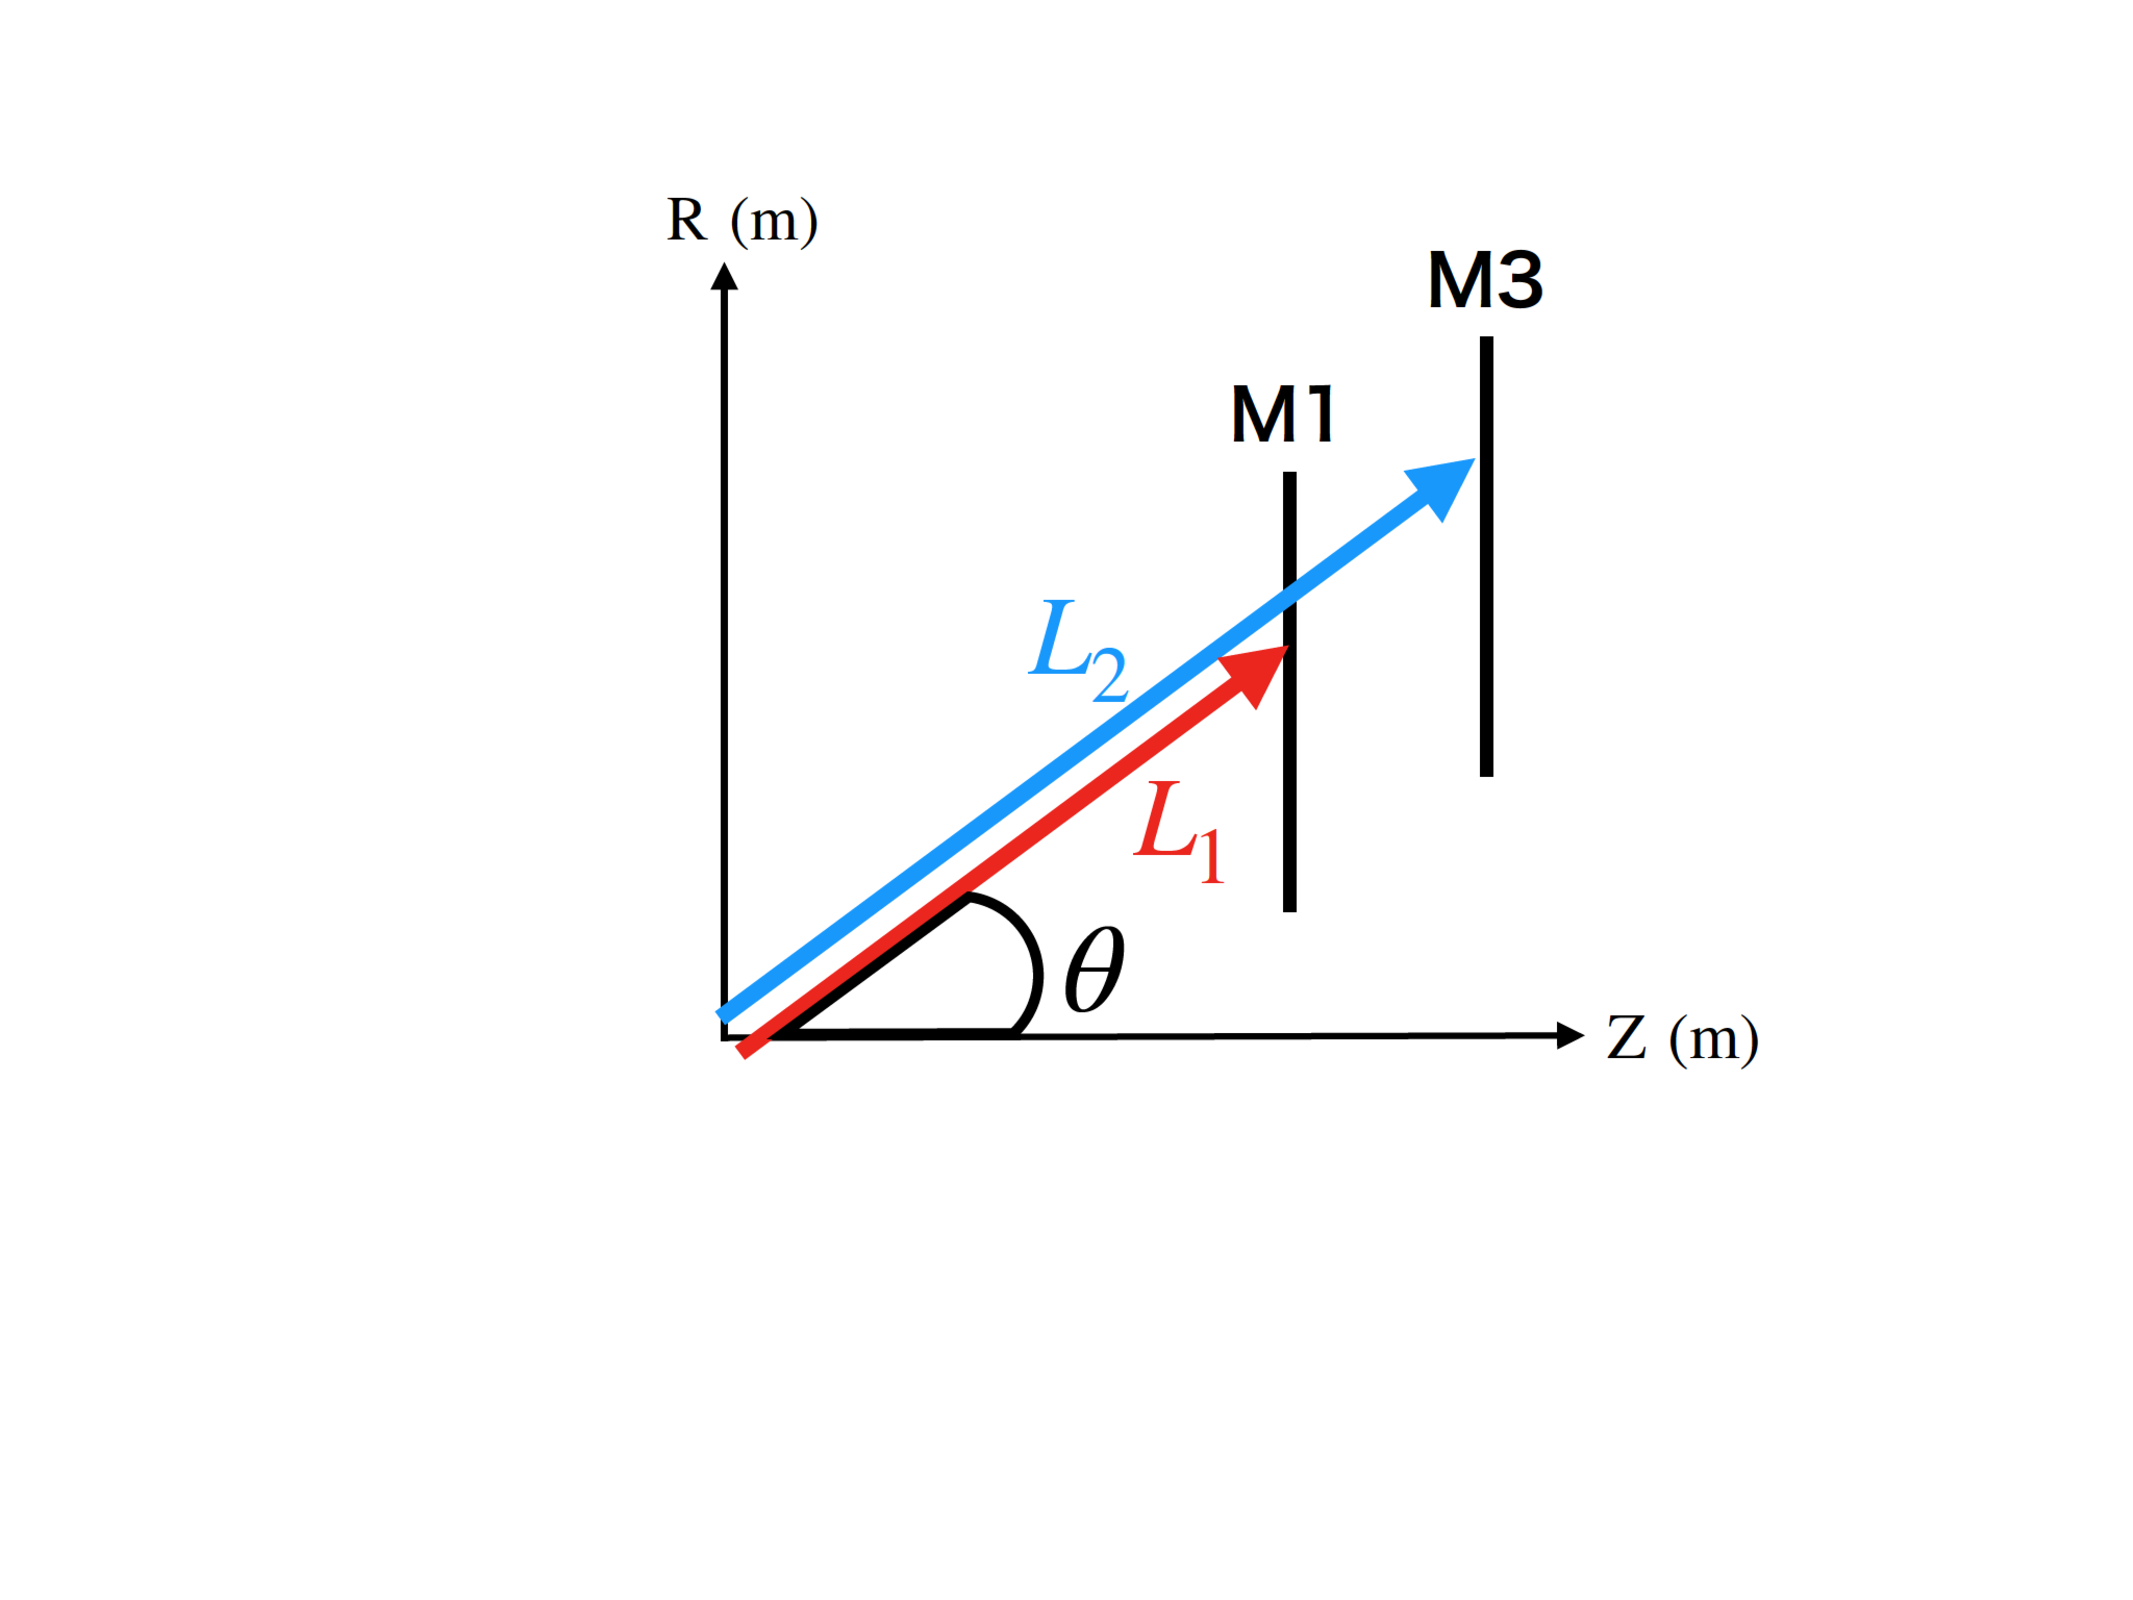
\includegraphics[width=0.7\textwidth,page=1]{img/slide/BX.pdf}
    \caption{衝突点から~TGC~検出器までの粒子到達の様子}\label{fig:velo}
\end{figure}

\begin{figure}[tbp]
    \begin{minipage}{0.33\hsize}
    \centering   
    \includegraphics[width=\textwidth,page=11]{img/rec/rec_e1.3_s.pdf}
    \end{minipage}
    \begin{minipage}{0.33\hsize}
    \centering   
    \includegraphics[width=\textwidth,page=9]{img/rec/rec_e1.3_s.pdf}
    \end{minipage}
    \begin{minipage}{0.33\hsize}
    \centering   
    \includegraphics[width=\textwidth,page=7]{img/rec/rec_e1.3_s.pdf}
    \end{minipage}\\
    \begin{minipage}{0.33\hsize}
    \centering   
    \includegraphics[width=\textwidth,page=11]{img/rec/rec_e2.2_s.pdf}
    \subcaption{}
    \end{minipage}
    \begin{minipage}{0.33\hsize}
    \centering   
    \includegraphics[width=\textwidth,page=9]{img/rec/rec_e2.2_s.pdf}
    \subcaption{}
    \end{minipage}
    \begin{minipage}{0.33\hsize}
    \centering   
    \includegraphics[width=\textwidth,page=7]{img/rec/rec_e2.2_s.pdf}
    \subcaption{}
    \end{minipage}
    \caption[粒子速度に依存した確率分布の変化]{粒子速度に依存した確率分布の変化。上図は$|\eta|=1.3$、下図は$|\eta|=2.2$の領域での分布を示している。赤が~M1~における確率分布、青が~M3~における確率分布を示している。(a)~$\beta=1.0$。(b)~$\beta=0.8$。(c)~$\beta=0.6$。}\label{fig:recbeta}
\end{figure}

\subsection{トリガー効率の算出}\label{sec:prot}
\figref{fig:recbeta}ではシミュレーションにおける速度による確率分布の変化について見積もった。$\beta=1.0$の場合は、\figref{fig:rectune}の分布と同じである。この図では、横軸の時間軸に対して、前バンチ、基準バンチ、次バンチのゲートが設定されている。従って、確率分布の三角形がどれだけの割合でバンチ識別のタイミングにおいてどこに位置しているのかを見積もることで、トリガーできる割合を間接的に算出することができる。基準バンチに含まれる割合がシングルミューオントリガーのトリガー効率となり、次バンチに含まれる割合が遅い荷電粒子探索用トリガーのトリガー効率となると考えられる。
\figref{fig:efftune}に$|\eta|=1.0$における\figref{fig:rectune}の確率分布より算出したトリガー効率を示す。ワイヤー、ストリップそれぞれにトリガー効率を算出し、効率を掛け合わせることによって全体のトリガー効率を見積もる。
次節では、上記の流れで見積もることができたトリガー効率をモンテカルロシミュレーションで得られた効率と比較し、トリガー効率の見積もり手法の評価を行う。
\begin{figure}[tbp]
    \begin{minipage}{0.49\hsize}
    \centering   
    \includegraphics[width=\textwidth,page=5]{img/rec/eff_wire.pdf}
    \subcaption{}
    \end{minipage}
    \begin{minipage}{0.49\hsize}
    \centering   
    \includegraphics[width=\textwidth,page=5]{img/rec/eff_strip.pdf}
    \subcaption{}
    \end{minipage} \\
    \begin{minipage}{0.99\hsize}
    \centering   
    \includegraphics[width=0.5\textwidth,page=5]{img/rec/eff_both.pdf}
    \subcaption{}
    \end{minipage}
    \caption[較正後のシミュレーションにおける見積もり手法を用いたトリガー効率の算出]{較正後のシミュレーションにおける見積もり手法を用いたトリガー効率の算出。赤は~L1~シングルミューオントリガー、青は遅い荷電粒子探索用トリガーを想定して見積もられたトリガー効率。(a)ワイヤーの確率分布から得られたトリガー効率。(b)~ストリップの確率分布から得られたトリガー効率。(c)~ワイヤー、ストリップのトリガー効率を掛け合わせ見積もった全体のトリガー効率。}\label{fig:efftune}
\end{figure}


\subsection{トリガー効率の見積もり手法の評価}\label{chap:caltri}
タイミング較正後のシミュレーションを利用して、粒子速度に依存したトリガー効率の見積もり手法の評価を行う。\figref{fig:comp}は、見積もり手法を利用して算出したトリガー効率とモンテカルロシミュレーションによって得られたデータから求めたトリガー効率の比較である。見積もり手法から得られたトリガー効率に関しては、シングルミューオントリガーおよび遅い荷電粒子用トリガーそれぞれおいてフルモンテカルロシミュレーションのトリガー効率を速度で積分した面積と一致するように較正している。$\beta$方向におけるトリガー可能な領域に良い一致がみられていることが分かる。この手法を用いて~Run~2~の実験データで期待されるトリガー効率を算出していく。

\begin{figure}[tbp]
    \centering   
    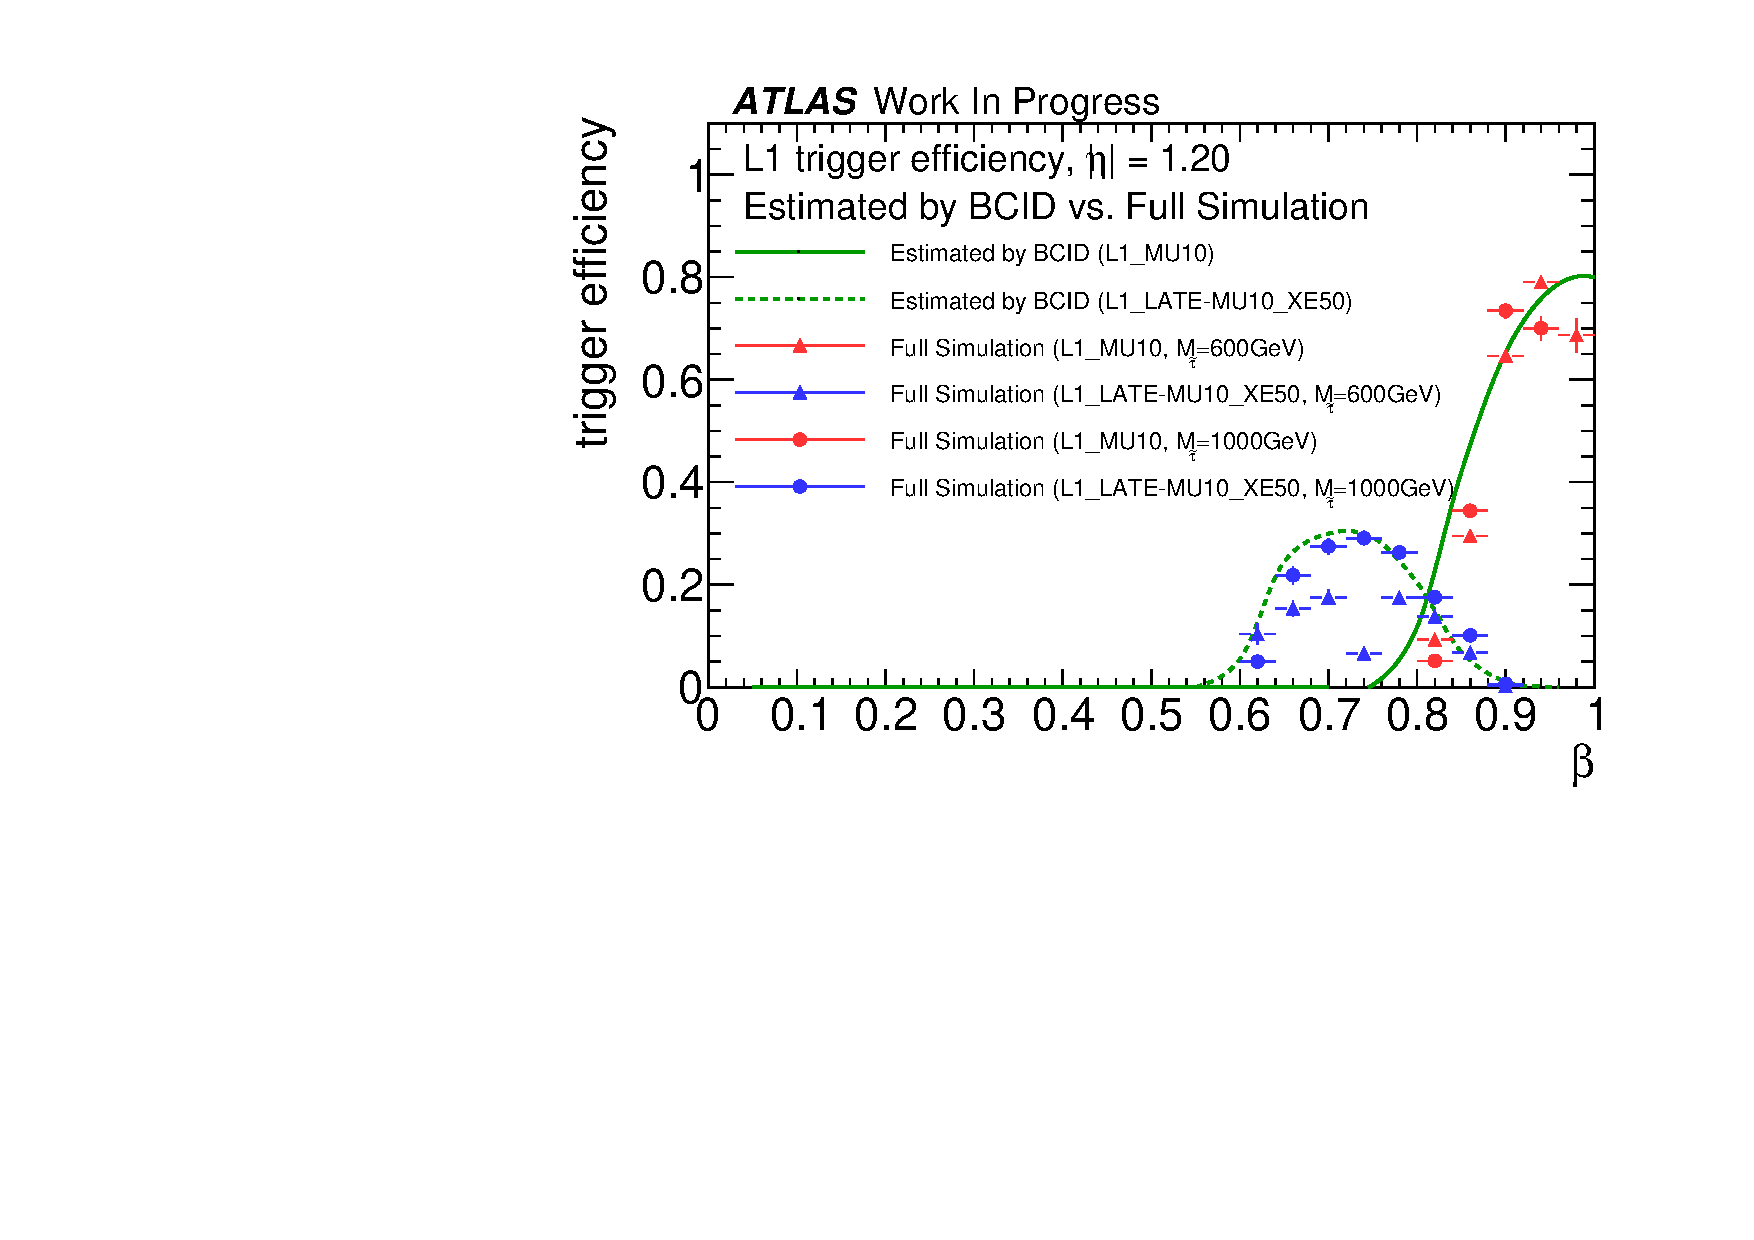
\includegraphics[width=\textwidth,page=1]{img/rec/vs.pdf}
    \caption[トリガー効率見積もり手法とフルモンテカルロシミュレーションのトリガー効率の比較]{トリガー効率見積もり手法とフルモンテカルロシミュレーションのトリガー効率の比較。緑の実線は見積もり手法から算出したシングルミューオントリガー、破線は遅い荷電粒子探索用トリガー、赤はフルモンテカルロシミュレーションにおけるシングルミューオントリガー、青は遅い荷電粒子探索用トリガーのトリガー効率を示す。▲はスタウサンプルの質量~600~GeV、●はスタウサンプルの質量~1000~GeV。}\label{fig:comp}
\end{figure}

\section{見積もり手法を利用したRun~2~の実験データとシミュレーションの比較}
\secref{sec:est}で説明したバンチ判定を利用したトリガー効率の見積もり手法を用いて、実際に~Run~2~のデータにおけるトリガー効率を算出する。シミュレーションを用いて得られたトリガー効率との差を比較することで、シミュレーションの評価を行う。
\subsection{確率分布関数の定義}
\secref{sec:pro}で説明した確率分布関数の定義方法を利用して、Run~2~の実験データおよびタイミング較正前後のシミュレーションにおける確率分布関数を定義する。定義のために必要なバンチ判定の分布には、\subsecref{chap:caltri}において記載した結果を利用している。確率分布関数の算出結果を\figref{fig:recall}に示す。実験データの確率分布はシミュレーションに対して分布の幅が大きいことが分かる。これはシミュレーションでの想定以上にデータにおけるタイミングにふらつきが生じていることを示唆している。より詳細に分布を再現するには\subsecref{subsec:cali}で述べた前のバンチを含めたタイミング較正等が必要となる。

実験データ、シミュレーションそれぞれに求めた確率分布関数をもとに、\secref{sec:prob}で述べた粒子速度に依存した確率分布の見積もりの計算を行い、トリガー効率を\secref{sec:prot}の要領で算出する。

\begin{figure}[tbp]
    \begin{minipage}{0.49\hsize}
    \centering   
    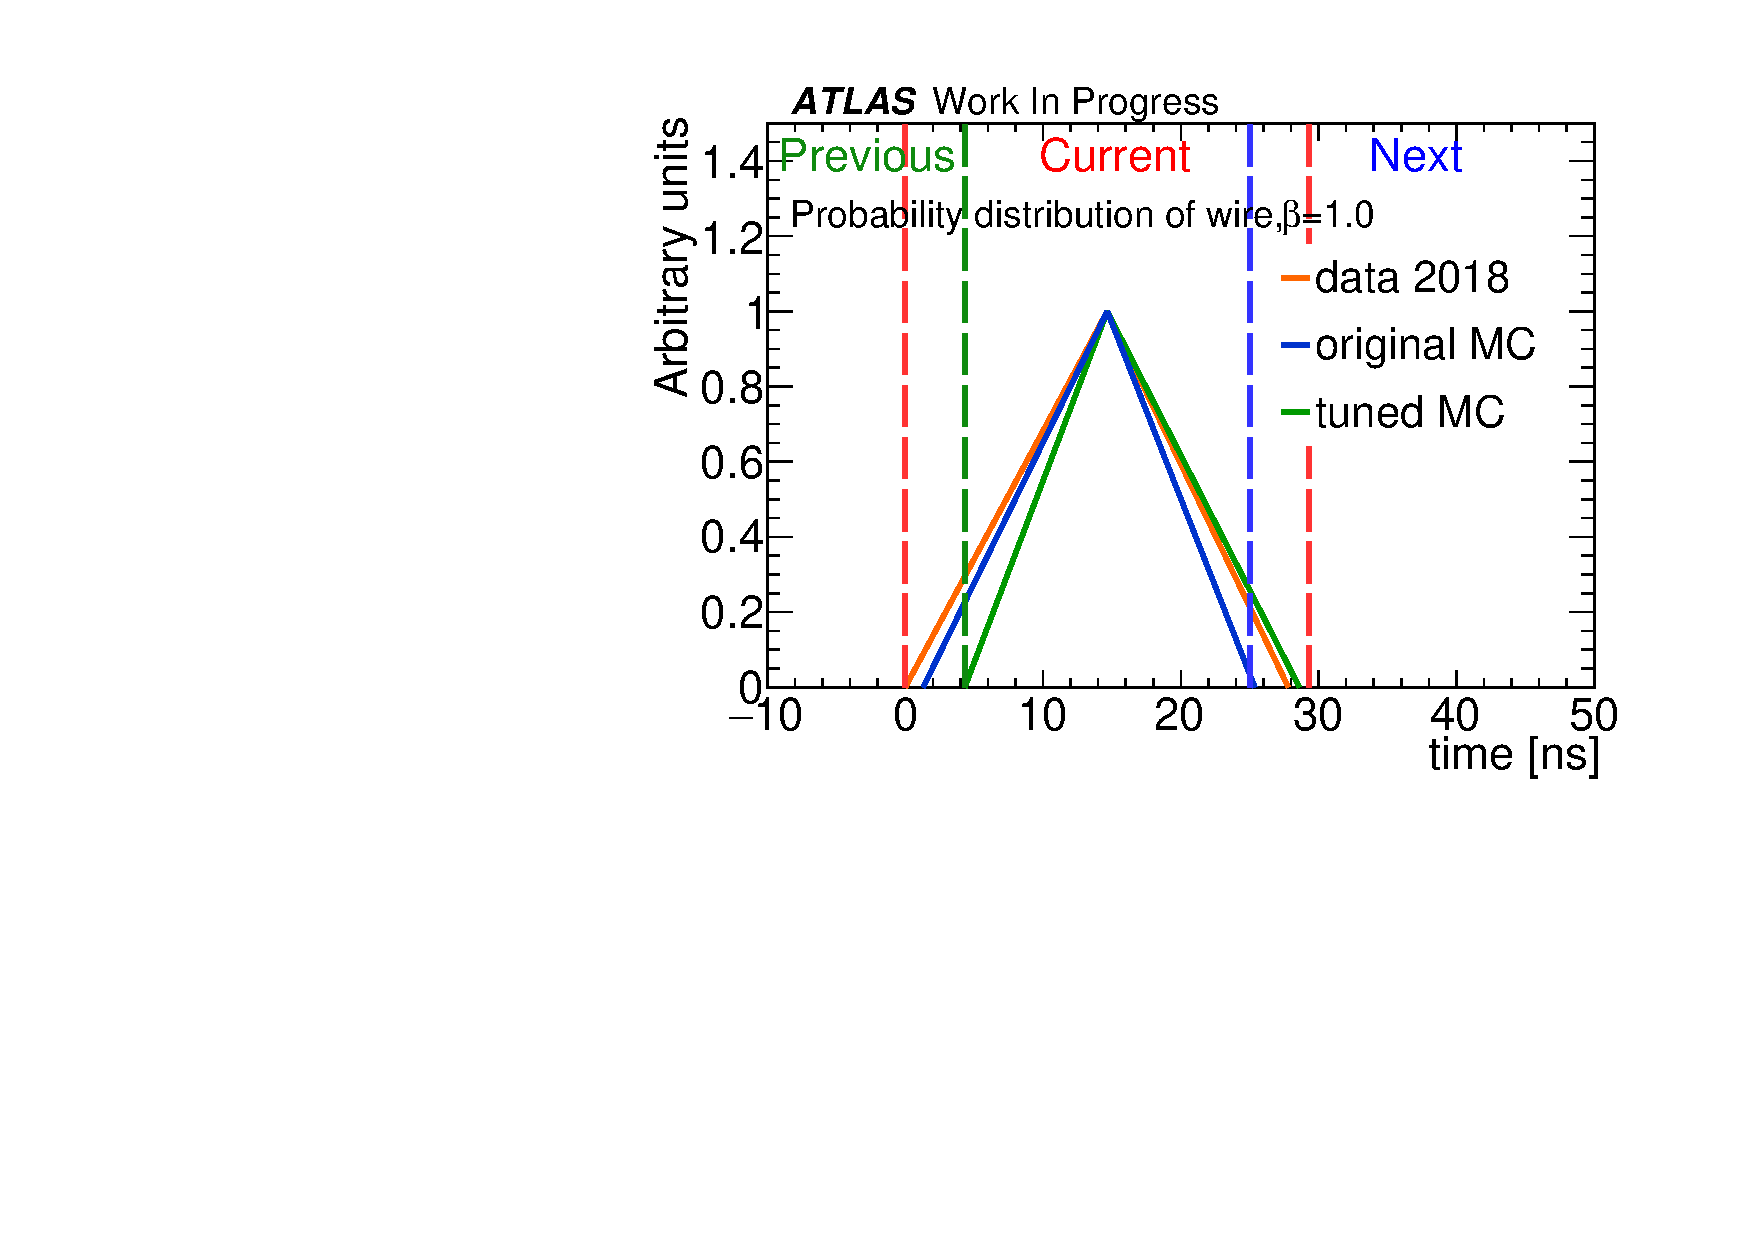
\includegraphics[width=\textwidth,page=1]{img/rec/recwire.pdf}
    \subcaption{}
    \end{minipage}
    \begin{minipage}{0.49\hsize}
    \centering   
    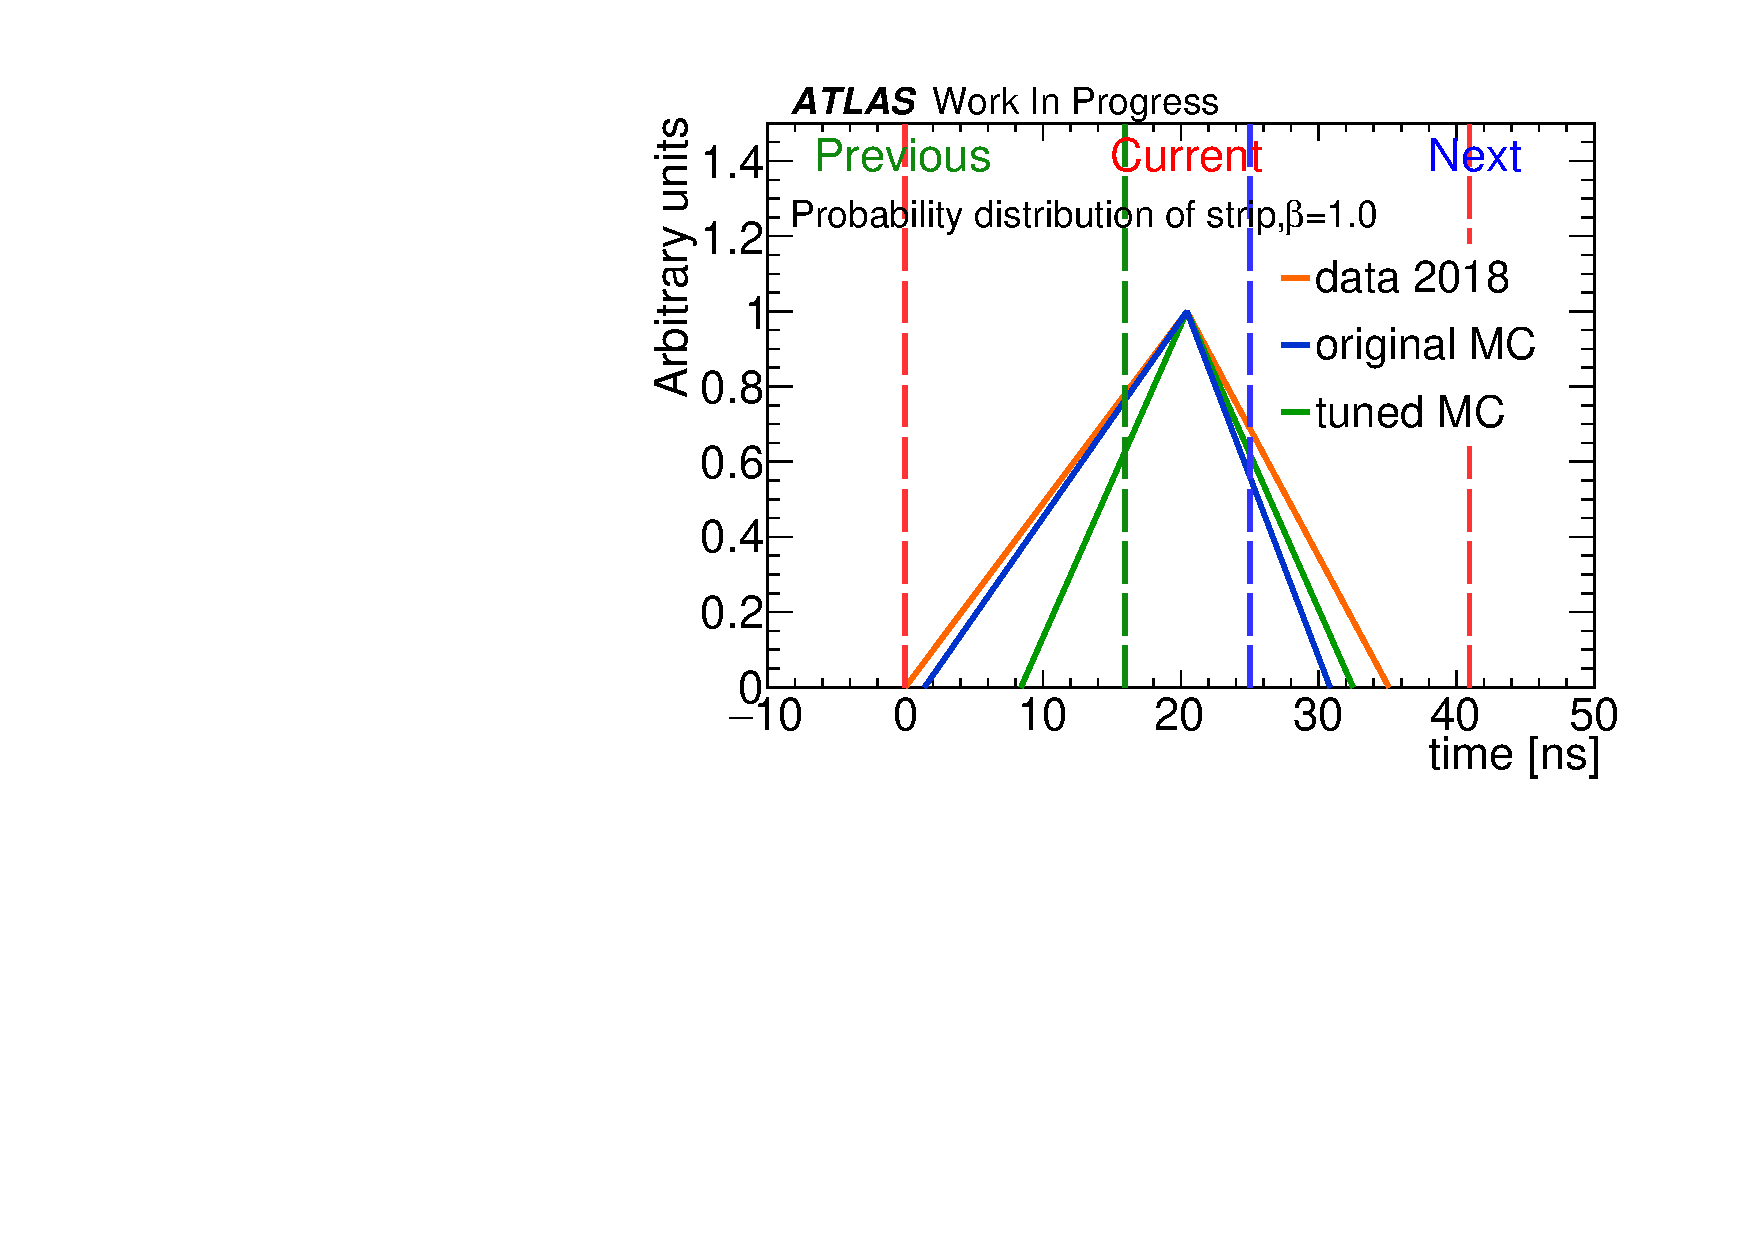
\includegraphics[width=\textwidth,page=1]{img/rec/recstrip.pdf}
    \subcaption{}
    \end{minipage}
    \caption[実験データおよびシミュレーションにおけるバンチ判定から推定したヒットタイミングの確率分布]{実験データおよびシミュレーションにおけるバンチ判定から推定したヒットタイミングの確率分布。橙色、緑色、青色はそれぞれ~Run~2~のデータ、改良後のシミュレーション、改良前のシミュレーションを表している。(a)~ワイヤーチャンネル。(b)~ストリップチャンネル。}\label{fig:recall}
\end{figure}

\subsection{見積もり手法を用いたトリガー効率の比較}
\figref{fig:rectritune}に見積もり手法により算出した~Run~2~の実験データおよび較正後のシミュレーションのトリガー効率と較正後のフルモンテカルロシミュレーションから算出したトリガー効率の比較を示す。
\begin{figure}[tbp]
    \centering   
    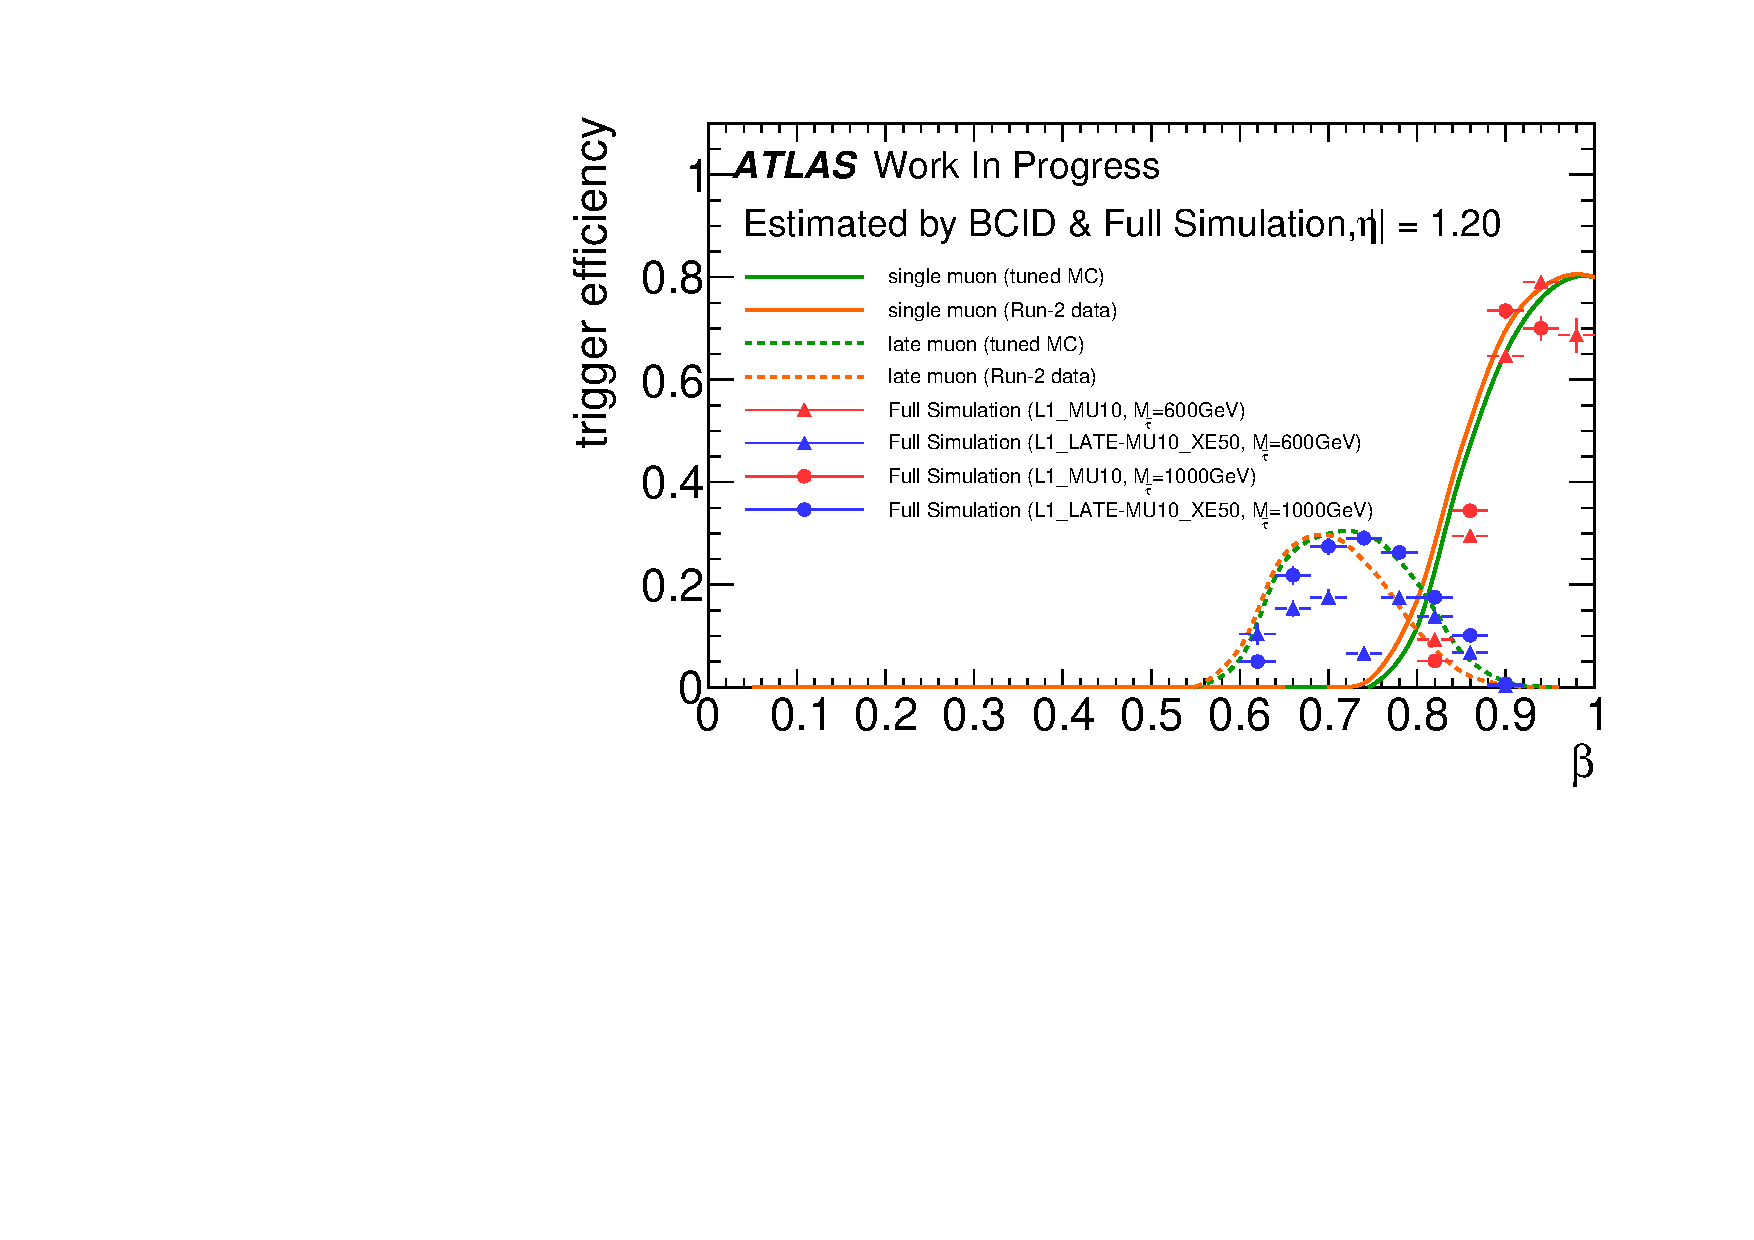
\includegraphics[width=\textwidth,page=1]{img/rec/tunetune.pdf}
    \caption[トリガー効率の見積もり手法から算出したシミュレーションおよび実験データにおけるトリガー効率とフルモンテカルロシミュレーションにおけるトリガー効率の比較]{トリガー効率の見積もり手法から算出したシミュレーションおよび実験データにおけるトリガー効率とフルモンテカルロシミュレーションにおけるトリガー効率の比較。$|\eta|=1.2$の領域におけるトリガー効率を算出している。実線はシングルミューオントリガー、破線は遅い荷電粒子探索用トリガーの見積もり手法から算出されたトリガー効率を示す。緑は較正後のシミュレーション、橙は~Run~2~の実験データを表す。点はフルモンテカルロシミュレーションによるトリガー効率を示し、赤はシングルミューオントリガー、青は遅い荷電粒子探索用トリガーのトリガー効率を示す。▲はスタウサンプルの質量~600~GeV、●はスタウサンプルの質量~1000~GeV。}\label{fig:rectritune}
\end{figure}
\subsecref{chap:caltri}で評価したように、フルモンテカルロシミュレーションのトリガー効率と見積もり手法から算出したシミュレーションにおけるトリガー効率には、取得できる粒子の速度に良い一致がみられる。また見積もり手法における~Run~2の実験データとシミュレーションの比較においては、シングルミューオントリガーではよい一致が確認できるが、遅い荷電粒子用トリガーにおいては少しの差異がみられている。これは\tbref{tb:tunebcidM1}で示したバンチ判定の前かつ基準バンチの割合の差異が確率分布関数の定義に変化を与えていることが影響していると考えられる。
\figref{fig:rectri}に~Run~2~における実験データおよびタイミング較正前後のシミュレーションそれぞれにおける見積もり手法をもとに算出したトリガー効率の比較を示す。実験データと較正後のシミュレーションにおいて遅い荷電粒子用トリガーの$0.7<\beta<0.9$の領域を除けばよい一致がみられている。
\begin{figure}[tbp]
    \centering   
    \includegraphics[width=\textwidth,page=4]{img/rec/est_eff.pdf}
    \caption[トリガー効率の見積もり手法から算出したシミュレーションおよび実験データにおけるトリガー効率の比較]{トリガー効率の見積もり手法から算出したシミュレーションおよび実験データにおけるトリガー効率の比較。$|\eta|=1.2$の領域におけるトリガー効率を算出している。実線はシングルミューオントリガー、破線は遅い荷電粒子探索用トリガーの見積もり手法から算出されたトリガー効率を示す。緑は較正後のシミュレーション、青は較正前のシミュレーション、橙は~Run~2~の実験データを表す。}\label{fig:rectri}
\end{figure}

物理解析においては実験データとシミュレーションの差異が系統的な不確かさに起因する。
本研究では実験データのトリガー効率を新たな見積もり手法で評価し、シミュレーションとの比較を行った。
シミュレーションを改良し実験データのタイミング調整を詳細に再現したことは不確かさを削減していることを示唆している。
バンチ判定分布を利用することで、新しい発想での粒子速度に依存したトリガー効率の評価方法を確立することに成功した。

本研究で用いた見積もり手法はヒットタイミングの確率分布関数の仮定から算出している。確率分布関数算出における仮定の正当性は、実際に~TGC~におけるヒット信号の時間分布の測定を行うことで担保できる。ATLAS~実験においてはヒット信号読み出し試験を行うための評価ボードの作成も進められている~\cite{ikemo}。評価ボードから得られた確率分布と本研究における確率分布を比較し正当性を評価することは今後の課題の一つである。

本研究では~TGC~検出器の詳細なタイミング較正を行った。実験データの新しいトリガー効率評価手法を確立し~Run~3~では重い長寿命荷電粒子探索のより不確かさの少ない物理解析が行えることが期待できる。
